\subsection{Classification scores}
\label{sec:classification_scores}
Even though we have taken many precautions with the purpose of maximizing the performance of the models, the actual results turned out to be quite disappointing. As a matter of fact, the classification reports in Tab. \ref{tab:report} show that the models are not able to correctly classify a great portion of the samples in the validation set.
\\The important thing to notice is that the lowest scores come from the classification of class 4, i.e. \textit{brake}. The reason for this is probably due to the fact that it is the least represented in the dataset, and therefore the models have not been able to learn the features that characterize them. This is confirmed by the fact that the results become proportionally better the higher the number of samples in the specific class, even though they are still far from being good.

\begin{table}[htbp]
    \centering
    
    \begin{subtable}{\textwidth}
        \centering
        \begin{tabular}{cccc}
            \toprule
            \textbf{Class} & \textbf{Precision} & \textbf{Recall} & \textbf{F1-score} \\
            \midrule
            0 & 0.24 & 0.47 & 0.31 \\
            1 & 0.38 & 0.58 & 0.46 \\
            2 & 0.52 & 0.68 & 0.59 \\
            3 & 0.87 & 0.68 & 0.76 \\
            4 & 0.05 & 0.08 & 0.06 \\
            \midrule
            \textbf{Accuracy} & & & 0.65 \\
            \textbf{Macro avg} & 0.41 & 0.50 & 0.44 \\
            \textbf{Weighted avg} & 0.72 & 0.65 & 0.67 \\
            \bottomrule
        \end{tabular}
        \caption{Model 0.}
    \end{subtable}
    \vspace{0cm}\\

    \begin{subtable}{\textwidth}
        \centering
        \begin{tabular}{cccc}
            \toprule
            \textbf{Class} & \textbf{Precision} & \textbf{Recall} & \textbf{F1-score} \\
            \midrule
            0 & 0.28 & 0.38 & 0.32 \\
            1 & 0.36 & 0.54 & 0.43 \\
            2 & 0.49 & 0.65 & 0.56 \\
            3 & 0.84 & 0.70 & 0.77 \\
            4 & 0.06 & 0.05 & 0.05 \\
            \midrule
            \textbf{Accuracy} & & & 0.65 \\
            \textbf{Macro Avg} & 0.40 & 0.46 & 0.43 \\
            \textbf{Weighted Avg} & 0.70 & 0.65 & 0.67 \\
            \bottomrule
        \end{tabular}
        \caption{Model 1.}
    \end{subtable}
    
    \caption{Classification reports of the two models, showing class-wise precision, recall and f1-score, and global accuracy over the validation set.}
    \label{tab:report}
\end{table}

\noindent The increased level of detail provided by confusion matrices (see Fig. \ref{fig:conf_mat}) does not tell a different story. However, it is way more useful when it comes to adjusting the models in order to make them drive in the Car Racing environment: for instance, steering left instead of braking on a straight is not as big of a deal as accelerating instead of braking when a curve is coming up.

\begin{figure}[htbp]
    \centering
    
    \subfloat[Model 0.]{
        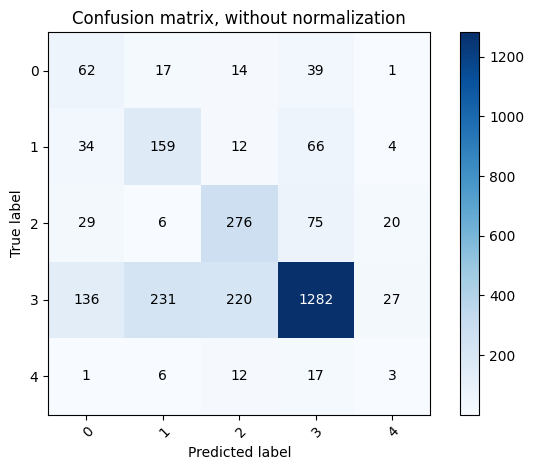
\includegraphics[width=0.4\textwidth]{figures/images/conf_mat_m0.png}
        \label{fig:conf_mat_m0}
    }
    \subfloat[Model 1.]{
        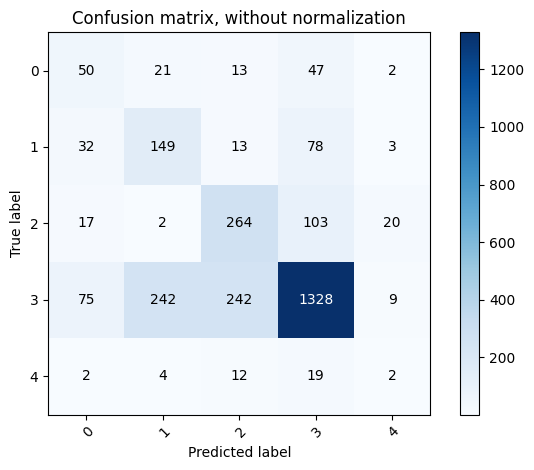
\includegraphics[width=0.4\textwidth]{figures/images/conf_mat_m1.png}
        \label{fig:conf_mat_m1}
    }

    \caption{Confusion matrices of the two models over the validation set.}
    \label{fig:conf_mat}
\end{figure}

\noindent \\After having tried with minimum improvement and considerable effort to obtain better performance by tuning the structures and the hyperparameters of the models (see Sec. \ref{sec:effect_of_class_weights}), the logical conclusion is that the dataset needs to be improved and possibly its split into training and validation sets needs to be changed and/or randomized.



